\chapter{文件系统模块的 Rust 重构}

\section{重构需求与总体设计}

Unix V6++ 的文件系统沿用 Unix V6 的基本组织方式。超级块记录空闲块和空闲 inode，磁盘 inode 保存文件元数据，内存 inode 承担缓存和同步职责，目录项把文件名映射到 inode 号，系统打开文件表和进程文件描述符表共同描述一次打开文件的状态。课程实验中经常观察的路径，包括 open、creat、link、unlink、read、write 和 stat，基本都围绕这些对象展开。

main 分支的 C++ 实现能够较直观地展示传统 Unix 文件系统，但内存 inode、File 对象和打开文件表之间的关系主要由裸指针、引用计数和调用约定维持。例如，路径解析过程中取得的 inode 需要在后续分支中正确释放，文件描述符复制后需要同步维护文件对象引用计数，错误返回路径还要避免遗漏已经取得的对象。这些约定在教学系统规模内可以工作，但不容易从类型接口中看出资源的实际归属。

refactor/x86 分支没有改变文件系统的磁盘格式，也没有替换 Unix V6 风格的目录项和多级块索引。重构主要把磁盘结构和内存控制信息分开表示，把 inode、File 和文件描述符之间的共享关系封装为可审查的引用类型，并把错误返回从全局状态和隐式约定转为 Result 与 PosixError 之间的显式转换。

实现中，超级块、inode、文件对象和目录项被重新写成 Rust 结构体或枚举；共享对象通过 \texttt{Arc<Spin<\_>>}、InodeRef、FileRef 和 Drop 逻辑管理。Clone 表示新增引用，Drop 表示离开作用域时减少引用，这种写法把“谁还持有对象”落实到类型行为中。错误处理则以 \texttt{Result<T, E>} 为主，内部错误在系统调用边界再映射为 ENOENT、EACCES、ENOSPC、EBADF 等 Unix 错误码。

Rust 版本文件系统主要由 src/fs.rs 及其下的 file\_system.rs、inode.rs、file.rs、open\_file\_manager.rs 和 file\_manager.rs 组成。其中，file\_system.rs 负责超级块和磁盘空间管理，inode.rs 负责 inode 对象及文件块访问逻辑，file.rs 负责文件对象和进程文件描述符表，open\_file\_manager.rs 负责系统打开文件表与内存 inode 表，file\_manager.rs负责路径解析和面向系统调用的文件操作流程。

模块关系可从一次 open 调用看出。FileManager 先完成路径解析和权限检查，再向 OpenFileTable 申请系统级 File 对象，并把它填入当前进程的 OpenFiles；若需要装载 inode，则通过 InodeTable 查找或分配内存 inode；真正读写磁盘块时，再进入 FileSystem 和缓冲区缓存。由此，系统调用层、文件对象层、inode 层和块设备层没有混在同一个函数中。

\begin{table}[htbp]
  \centering
  \caption{文件系统子模块功能说明表}\label{tab:fs-modules}
  \begin{tabular}{p{0.30\textwidth}p{0.60\textwidth}}
    \toprule
    \textbf{代表文件} & \textbf{主要功能} \\
    \midrule
    fs.rs & 组织并导出文件系统相关子模块，对外提供统一的文件系统系统调用入口 \\
    fs/file\_system.rs & 管理超级块、挂载表、空闲块和空闲 inode，负责文件系统装载、更新、空间分配与回收 \\
    fs/inode.rs & 定义内存 inode 与磁盘 inode 结构，实现文件读写、块映射、索引块访问和 inode 状态维护 \\
    fs/file.rs & 定义文件对象、进程文件描述符表和 I/O 参数结构，维护文件偏移、打开标志和引用关系 \\
    fs/open\_file\_manager.rs & 管理系统打开文件表和内存 inode 表，负责文件对象与 inode 对象的分配、共享和释放 \\
    fs/file\_manager.rs & 实现路径解析、目录查找、文件创建删除、权限检查以及面向系统调用的文件操作流程 \\
    dev/buffer\_manager.rs & 为文件系统提供缓冲区缓存支持，负责块缓存获取、读写、回收和同步 \\
    dev/buffer.rs & 定义缓冲区对象、逻辑块号和物理块号等基础类型，为文件系统块访问提供底层表示 \\
    \bottomrule
  \end{tabular}
\end{table}

\section{文件系统核心数据结构重构}

超级块被拆成磁盘表示和内存表示。DiskSuperBlock 对应磁盘上的固定布局，字段顺序和大小需要与镜像格式保持一致；SuperBlock 则是内核运行时使用的对象，除空闲块表、空闲 inode 表和时间信息外，还保存只读标志、修改标志以及空闲表锁。两者分开后，写回磁盘时只需要处理可持久化字段，运行时同步状态不会意外进入磁盘结构。

空闲块表锁和空闲 inode 表锁由 SleepFlag 表示。锁定、解锁和等待通道不再由外部代码直接改写字段，而是通过方法调用完成。load\_super\_block、write\_super\_block 和 update 集中处理超级块读入、修改和写回，其他模块通常只通过分配和释放接口接触超级块状态。

内存 inode 仍是文件系统运行时最频繁使用的对象。Inode 保留状态标志、文件模式、引用计数、设备号、inode 号、文件大小和块地址表等字段；InodeFlag 和 InodeMode 使用 bitflags 定义，避免在代码中反复出现难以辨认的整数掩码。权限检查、文件类型判断和脏标记更新因此可以写成围绕标志位类型的方法或组合判断。

inode 生命周期改动较大。InodeSlot 表示表中的一个槽位，InodeRef 表示可共享的持有关系，InodeRefGuard 用于 i\_get 返回后的临时持有场景。InodeRef 被克隆时增加引用计数，离开作用域时由 Drop 触发减少计数；InodeRefGuard 则避免路径解析中“刚取得 inode 又被提前释放”的情况。配合 InodeTable 的 i\_get、i\_dup 和 i\_put\_slot，inode 的装载、共享和回收不再完全依赖调用者记忆释放顺序。

打开文件对象采用相同思路。File 保存打开标志、引用计数、关联 inode 和当前偏移量；FileSlot 对应系统打开文件表中的槽位，FileRef 对应一次持有。dup、fork 后的文件描述符共享同一个 FileRef 语义对象，close 时由引用计数决定是否真正释放底层 File。读写偏移量仍属于 File，而不是进程文件描述符，因此共享描述符的偏移行为与 Unix 语义一致。

OpenFileTable 只关心系统范围内哪些 File 可用，OpenFiles 只关心当前进程的文件描述符到 FileRef 的映射。文件打开时，两张表分别分配槽位；文件关闭时，进程表先去掉描述符，再由 FileRef 的释放逻辑处理系统级对象。这一层次与原系统一致。异常返回时，只要临时对象离开作用域，已经取得的引用就会按同一规则回收。

\begin{table}[htbp]
  \centering
  \caption{核心数据结构功能对照表}\label{tab:fs-structures}
  \begin{tabular}{p{0.28\textwidth}p{0.62\textwidth}}
    \toprule
    \textbf{数据结构} & \textbf{主要职责} \\
    \midrule
    SuperBlock & 表示内存中的超级块，维护空闲块表、空闲 inode 表、修改状态和只读状态 \\
    DiskSuperBlock & 表示磁盘上的超级块布局，用于超级块的装载与写回 \\
    Mount & 记录设备号、超级块和挂载点 inode，用于描述已装载文件系统 \\
    Inode & 表示内存 inode，维护文件类型、权限、大小、块地址表、引用计数和状态标志 \\
    DiskInode & 表示磁盘 inode 布局，用于磁盘 inode 和内存 inode 之间的数据转换 \\
    InodeTable & 管理系统中的内存 inode 缓存，负责 inode 装载、复用、引用计数和释放 \\
    InodeRef & 对内存 inode 的引用封装，通过克隆和析构配合引用计数管理生命周期 \\
    InodeRefGuard & 对临时持有的 inode 引用进行保护，控制某些场景下的释放时机 \\
    File & 表示系统打开文件对象，记录打开标志、引用计数、关联 inode 和当前文件偏移 \\
    OpenFileTable & 管理系统范围内的文件对象数组，为进程分配可共享的打开文件对象 \\
    OpenFiles & 表示进程级文件描述符表，维护文件描述符到文件对象的映射关系 \\
    FileRef & 对文件对象的引用封装，通过自动增加和减少计数实现共享管理 \\
    DirectoryEntry & 表示目录项，保存文件名和对应 inode 编号，用于路径解析和目录遍历 \\
    IOParameter & 保存一次文件读写过程中的用户缓冲区地址、偏移量和剩余字节数 \\
    \bottomrule
  \end{tabular}
\end{table}

\section{文件系统核心功能实现}

DirectoryEntry 仍由固定长度文件名和 inode 号组成，这保证了磁盘目录格式与原系统兼容。路径解析由 FileManager::find 及其下层搜索逻辑完成。绝对路径从根 inode 开始，相对路径从当前工作目录开始；每解析一个路径分量，就在当前目录文件中顺序查找对应目录项；查找模式决定最后一级是返回已有 inode、保留空目录项用于创建，还是定位待删除项。

\begin{figure}[htbp]
  \centering
  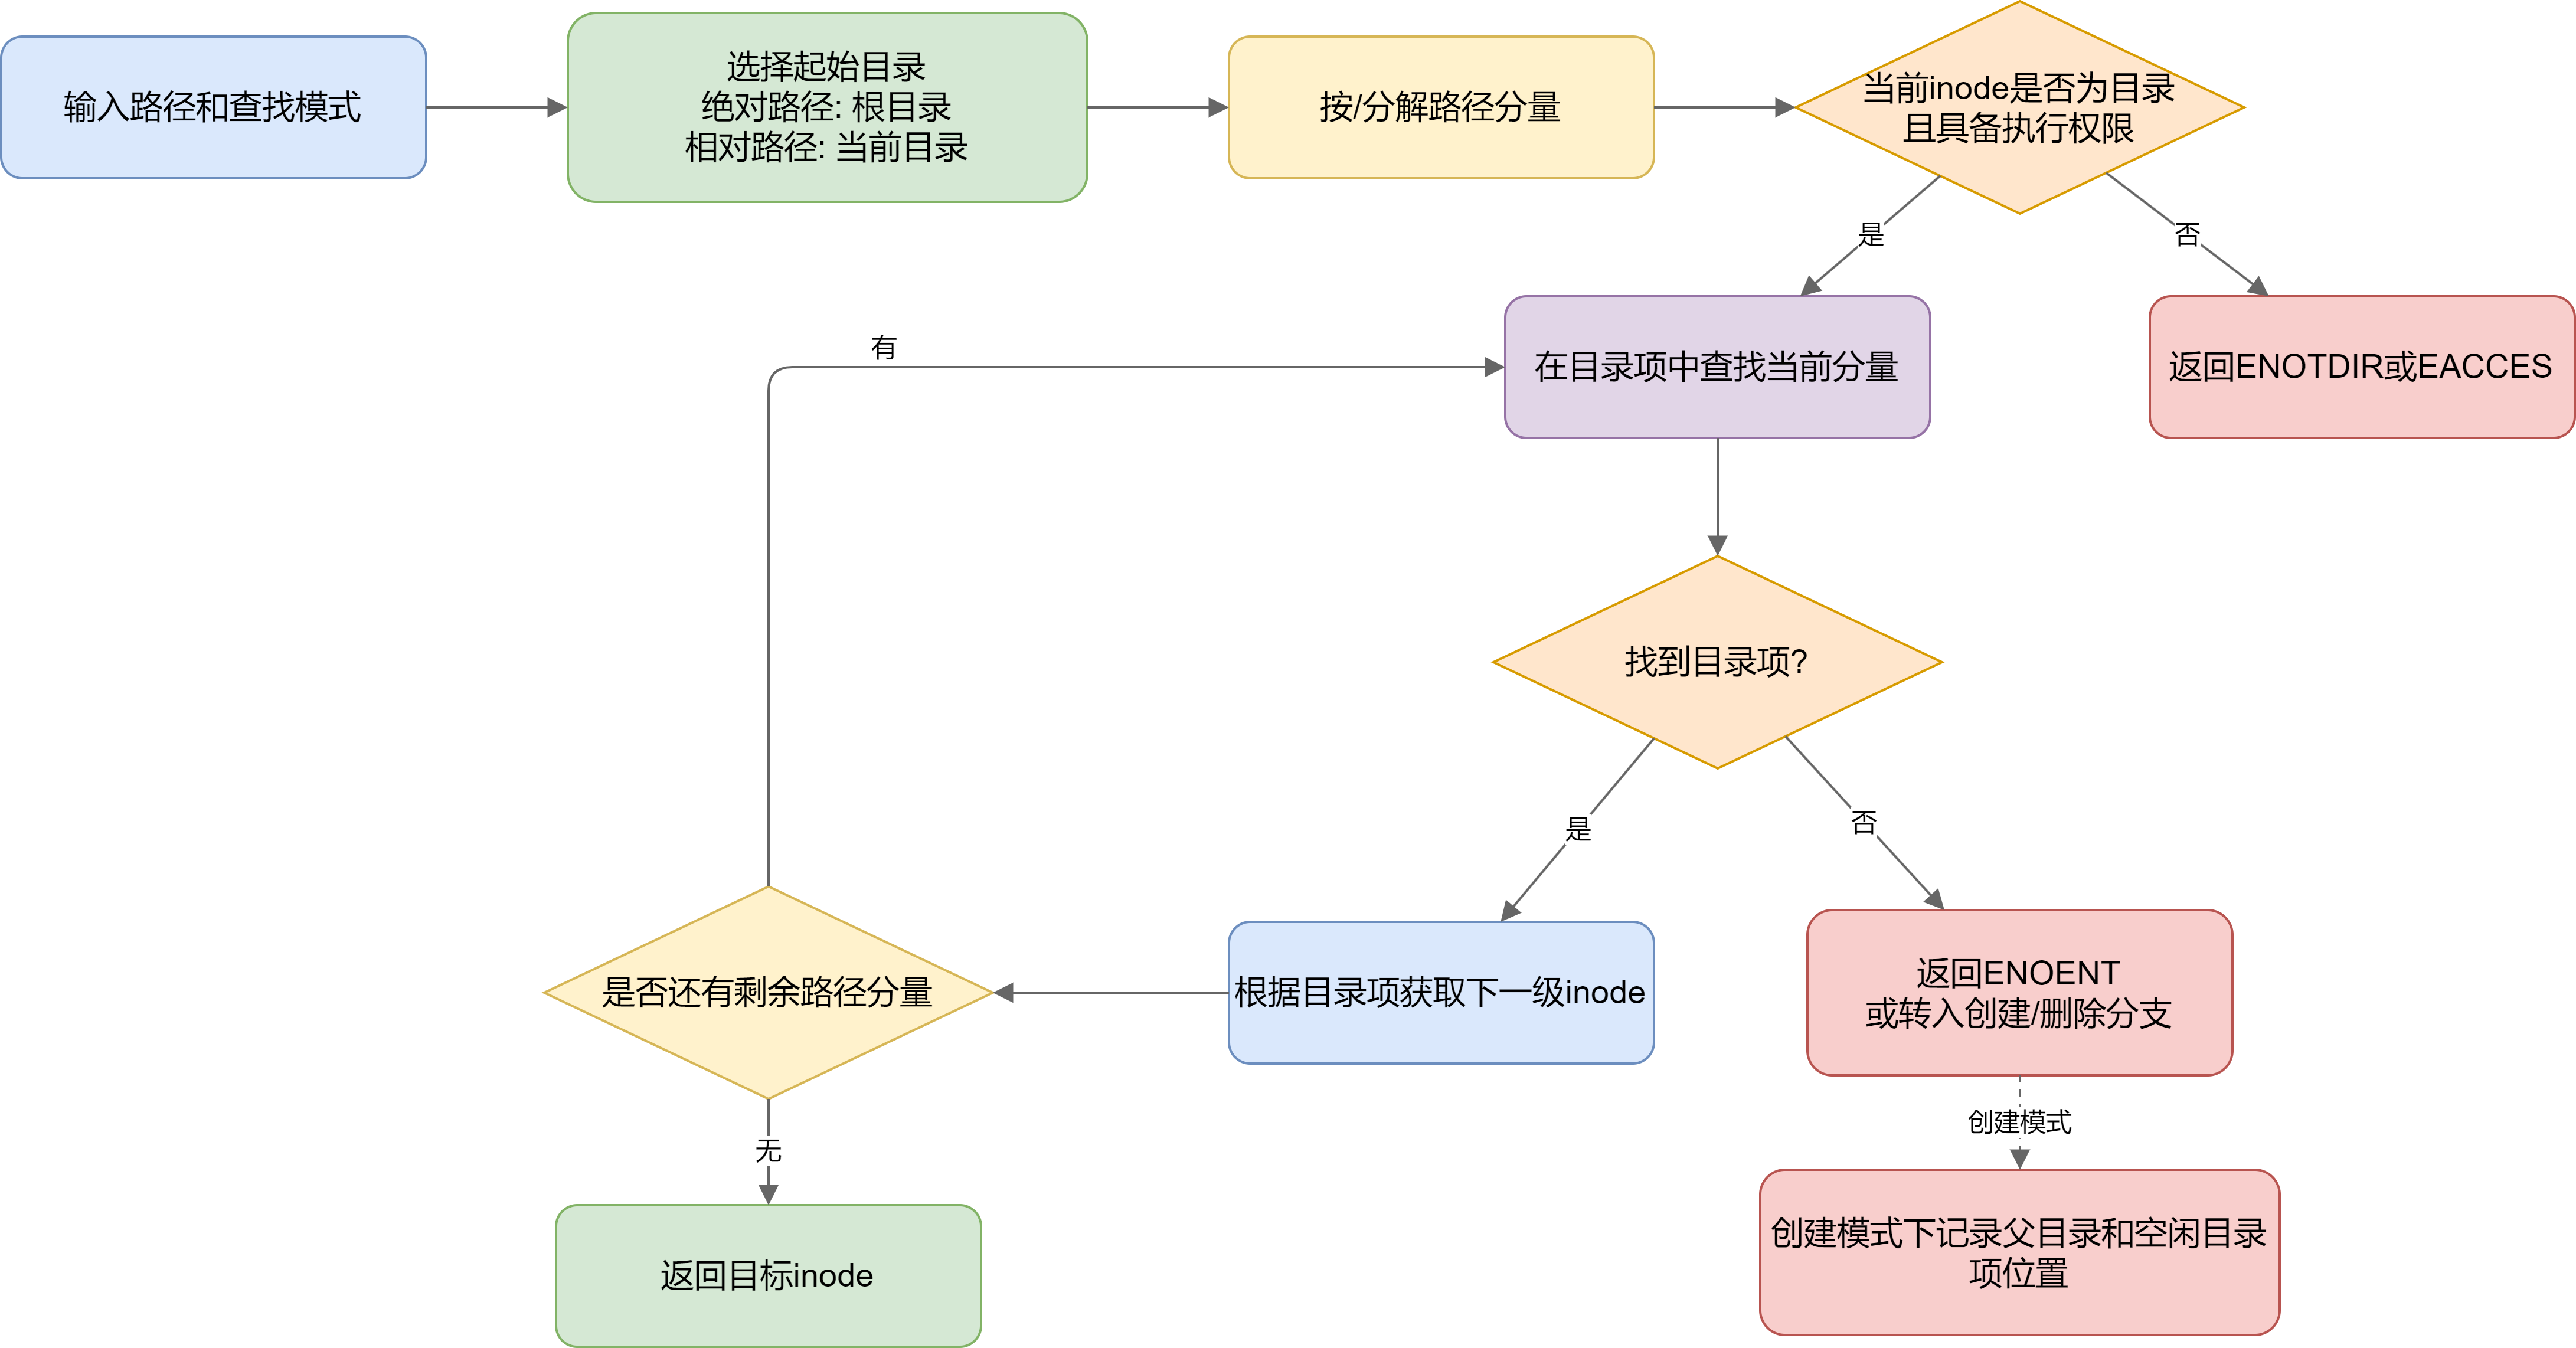
\includegraphics[width=0.72\textwidth]{figures/4/1路径解析.png}
  \caption{路径解析流程图}
\end{figure}

实现上，目录遍历、权限检查和目录项搜索被放入 InodeRefExt trait 及其 search 方法。这样写的好处不是改变算法，而是把“目录 inode 可以执行搜索”这一事实放到接口上表达。search 执行过程中还会维护目录项缓冲和偏移量信息，后续 creat、link、unlink 可以复用这些上下文，而不必重新扫描同一目录。

文件读写路径由 FileRef、Inode 和缓冲区缓存串联。FileManager 根据文件描述符取得 FileRef，检查 FileFlags 后读取或更新文件偏移量；Inode 根据逻辑块号找到物理块，并通过缓冲区缓存完成块读写；写入超过原文件大小时，inode 负责更新文件长度和修改标志。这一分工使文件偏移、文件元数据和块缓存状态分别落在对应对象中。

读操作按照当前偏移和剩余长度逐块推进，顺序访问时可以触发预读。写操作在目标逻辑块尚未分配时申请新块，并根据写入范围选择读后改写、延迟写或异步写。字符设备和块设备文件仍通过同一 read/write 系统调用进入，但在 inode 打开和读写阶段根据文件类型分流到设备接口。

块映射逻辑集中在 Inode::get\_blk 及相关辅助函数中。小文件直接使用 inode 地址表中的块号；文件增大后进入一次间接块；继续扩大时再进入二次间接块。若目标块尚未分配，函数会通过 FileSystem 的空闲块分配接口申请新块，并更新 inode 地址表或间接块内容。这个过程仍是 Unix V6 风格的块索引，只是 Rust 版本把直接块、一次间接块和二次间接块的处理路径拆得更清楚。

\begin{figure}[htbp]
  \centering
  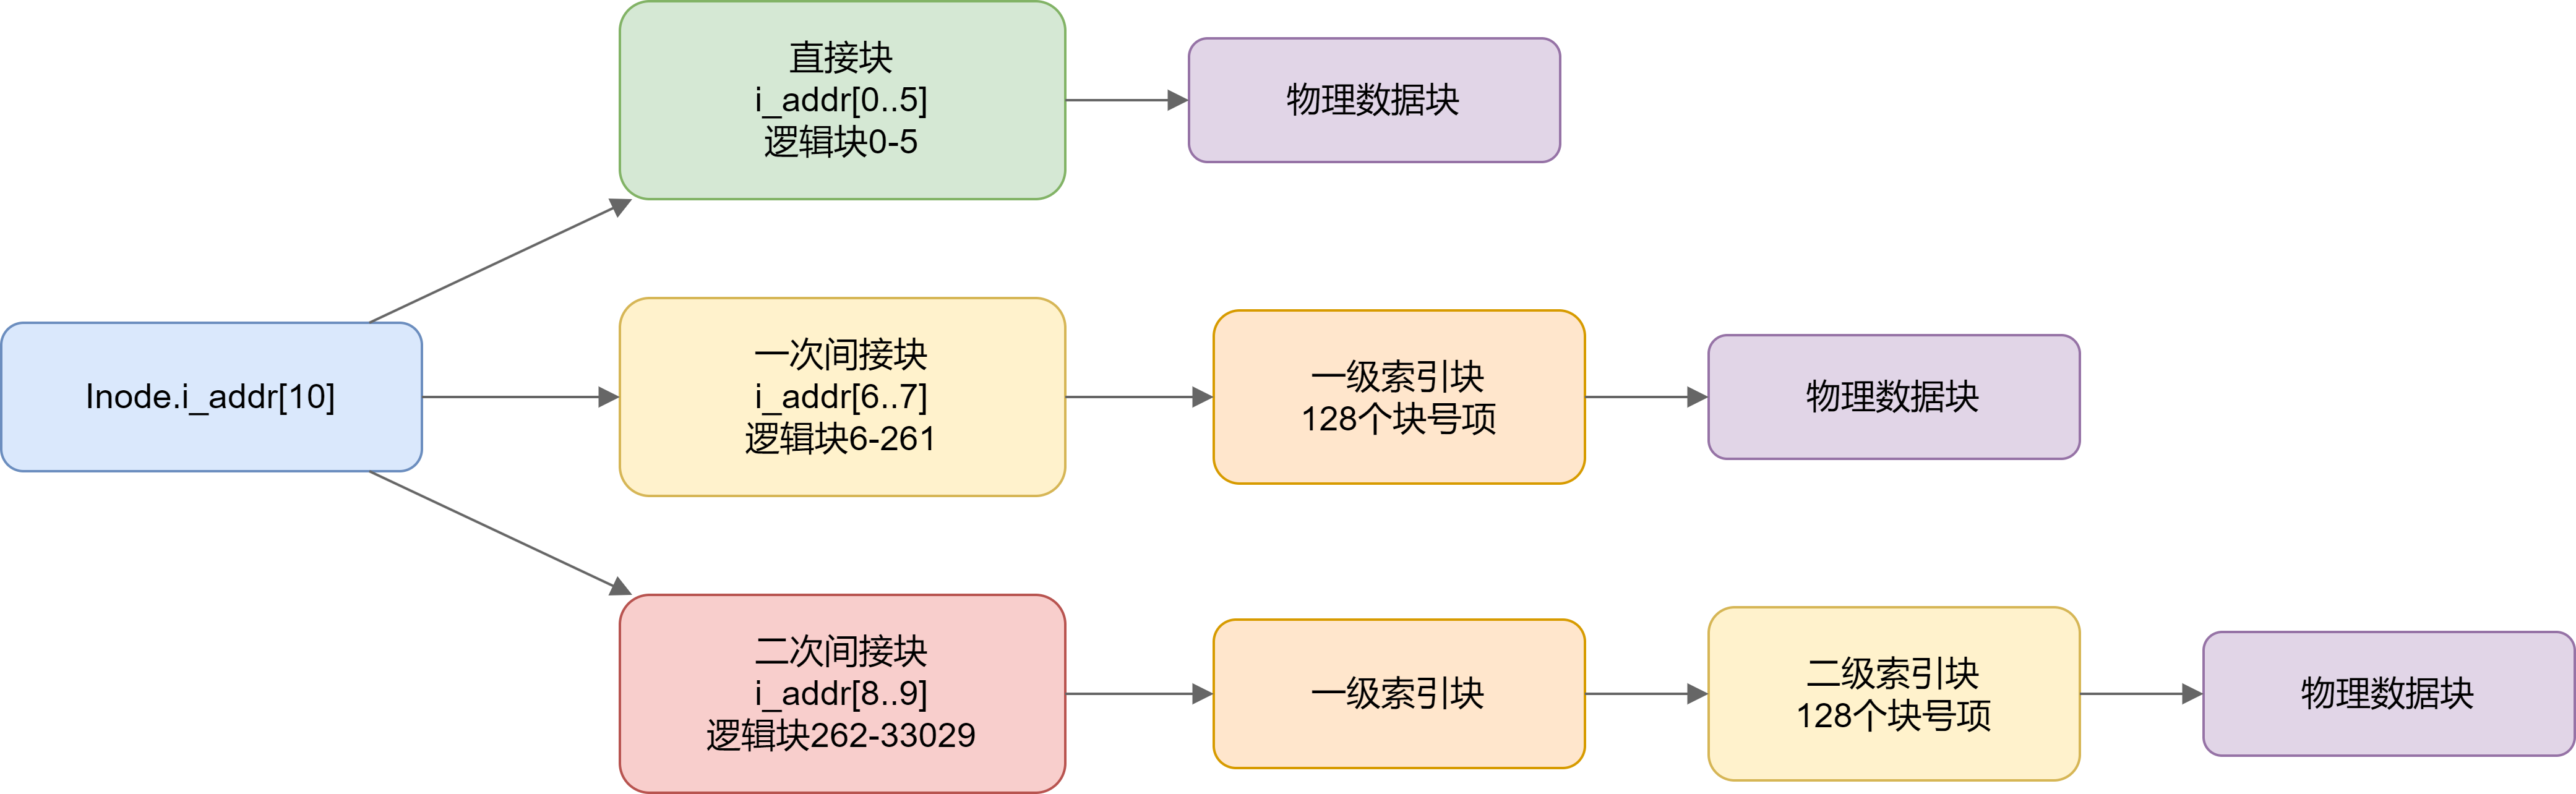
\includegraphics[width=0.68\textwidth]{figures/4/2块映射.png}
  \caption{块映射机制示意图}
\end{figure}

这里没有引入位图或 extent 等新结构，原因是本课题希望保持原教学文件系统的可比性。类型化块号和显式 Buffer 对象主要用于减少误把逻辑块号、物理块号和缓冲区数据混用的机会，而不是改变磁盘布局。

用户程序看到的仍是 Unix 风格系统调用。src/fs.rs 导出 open、close、creat、link、unlink、chdir、stat、seek、dup、pipe 等入口；interrupt/system\_call.rs 在陷入内核后按系统调用号分发。文件系统不直接处理 trap 现场，而是接收已经解析出的调用请求，并把返回值或错误码交回系统调用层。

这种边界对调试有实际意义。系统调用参数复制或用户地址检查出错时，问题通常在系统调用层；路径解析、inode 引用或块分配出错时，问题则落在 FileManager、InodeTable 或 FileSystem。分层后，错误码虽然仍按 Unix 语义返回，但错误来源更容易追踪。

\section{错误处理与安全性分析}

文件系统内部大量函数返回 \texttt{Result<T, E>}。超级块装载可能失败，inode 获取可能因为表满失败，路径查找可能返回 ENOENT，块分配可能返回 ENOSPC，用户缓冲区复制也可能返回 EFAULT。把这些情况写入返回类型后，调用者不能在类型层面忽略失败分支。

这一点在 open 和 creat 路径中较明显。函数可能已经取得父目录 inode、分配了系统文件对象，随后又在权限检查、目录项写入或 inode 分配处失败。如果继续沿用分散的错误约定，回收顺序容易与正常路径混杂。Result 与 RAII 结合后，错误向上传播时，临时引用会随作用域退出自动释放，真正需要手工处理的只剩下磁盘状态更新和错误码映射。

同时，尽管内部大量采用 Rust 风格的错误返回方式，但模块对外仍需维持 Unix兼容的错误语义。因此，Rust 版本保留了 PosixError 枚举，用于表示 ENOENT、EACCES、ENOSPC、EBADF、EROFS 等常见错误。文件系统内部的专用错误类型，如 FileSystemError 和缓冲区错误，在需要对外暴露时会进一步映射为 PosixError，再通过系统调用入口写回用户态。

内部错误不必一开始就压缩成 POSIX 错误码。例如，空闲块不足、inode 表不可用和缓冲区 I/O 失败在内部可以区分；到系统调用边界时，再统一转换为用户态程序理解的返回值。这种处理既保留调试信息，也没有破坏原系统接口。

资源管理的主要收益来自引用关系被显式化。inode 和 File 都存在跨模块共享，C++ 版本依靠调用者配对执行增加、减少计数；Rust 版本把这类操作收进 InodeRef、FileRef 和 Drop。需要强调的是，内核代码仍有 unsafe 边界和全局对象，Rust 并不会自动消除所有问题；但在文件系统主体逻辑中，引用数量和释放时机已经比原来更容易审查。

从维护角度看，超级块、inode、File、OpenFileTable、OpenFiles 和 FileManager 的职责边界比 main 分支更容易区分。底层块访问和同步仍由缓冲区缓存承担，设备错误也仍可能向上传播；文件系统层的改动主要在于把对象关系和错误出口收束到较少的接口上。

\section{文件系统主体小结}

本章围绕文件系统的 Rust 重构展开。磁盘格式、目录项结构和多级块索引保持 Unix V6++ 原有逻辑，重构重点放在内存表示、引用关系和错误路径上。InodeRef、FileRef、InodeRefGuard、Result 和 PosixError 共同承担了原先由裸指针、全局状态和调用约定维持的部分责任。经过这些调整，文件系统仍能呈现原有教学机制，同时更便于检查 inode、文件对象和缓冲区之间的资源关系。
